\begin{frame}{目录}
    \tableofcontents
\end{frame}

\begin{section}{值函数近似方法\alert{(Deep Q-Learning)}}

\begin{frame}{从表格表示到函数表示}
    \begin{figure}
        \centering
        \includegraphics[width=0.6\textwidth]{assets/Figure_chapterMap.png}
    \end{figure}
\end{frame}

\begin{frame}{从表格表示到函数表示}
    直到现在本节课涉及的所有动作价值和状态价值都是用\alert{表格}表示的。
    \begin{itemize}
        \item 状态价值:
        \begin{table}[]
            \begin{tabular}{@{}ccccc@{}}
            \toprule
            State & $s_1$& $s_2$& $\cdots$& $s_n$\\ \midrule
            Value & $v_\pi(s_1)$& $v_\pi(s_2)$& $\cdots$& $v_\pi(s_n)$\\
            \bottomrule
            \end{tabular}
        \end{table}
        \item 动作价值:
        \begin{table}[]
            \begin{tabular}{@{}cccccc@{}}
            \toprule
             & $a_1$& $a_2$& $a_3$& $a_4$& $a_5$\\ \midrule
            $s_1$ & $q_\pi(s_1,a_1)$& $q_\pi(s_1,a_2)$& $q_\pi(s_1,a_3)$& $q_\pi(s_1,a_4)$& $q_\pi(s_1,a_5)$\\
            $\vdots$ &&&$\vdots$&&  \\
            $s_9$  & $q_\pi(s_9,a_1)$& $q_\pi(s_9,a_2)$& $q_\pi(s_9,a_3)$& $q_\pi(s_9,a_4)$& $q_\pi(s_9,a_5)$\\
            \bottomrule
            \end{tabular}
        \end{table}
        \item \alert{优势}:直观,更容易理解分析
        \item \alert{缺点}:难以应对大且\alert{连续}的状态空间。
        
        主要体现在两点:1)存储空间;2)泛化能力。
    \end{itemize}
\end{frame}

\begin{frame}{从表格表示到函数表示}
    比如,我们可以用一条直线来拟合所有的状态价值:
    \begin{figure}
        \begin{tikzpicture}
            \draw[->] (0,0) -- (5,0) node[right] {$s$};
            \draw[->] (0,0) -- (0,3) node[above] {$v_\pi(s)$};
            \draw[domain=0:4,smooth,variable=\x] plot ({\x},{0.5*\x+0.5});
            
            % 补充的点
            \filldraw (1,1.2) circle (2pt) node[above left] {};
            \filldraw (2,1.3) circle (2pt) node[above left] {};
            \filldraw (3,2.3) circle (2pt) node[above left] {};
            \filldraw (4,2.2) circle (2pt) node[above left] {};

            % 在直线末端添加方程
            \node at (4.8,3) {$\hat{v}(s) = as + b$};

            % 补充坐标轴上的信息
            \draw[dashed] (1,0) -- (1,1.2) node[below] at (1,0) {$s_1$};
            \draw[dashed] (2,0) -- (2,1.3) node[below] at (2,0) {$s_2$};
            \draw[dashed] (3,0) -- (3,2.3) node[below] at (3,0) {$s_3$};
            \draw[dashed] (4,0) -- (4,2.2) node[below] at (4,0) {$s_4$};
        \end{tikzpicture}
    \end{figure}
    比如这条直线的方程是:
    \[
        \hat{v}(s,w)=as+b=[s,1]\begin{bmatrix}
            a \\
            b \\
        \end{bmatrix}=\phi^T(s)w
    \]
    其中$w$是参数向量;$\phi(s)$是特征向量;$\hat{v}(s,w)$关于$w$是线性的。
\end{frame}

\begin{frame}{从表格表示到函数表示}
    表格表示和函数表示有什么区别?
    \begin{itemize}
        \item 获取数据的方式不同:
        \begin{itemize}
            \item 表格:将行列作为索引,直接去表中查得相应数据
            \item 函数:需要输入特征向量计算:$s\rightarrow\phi(s)\rightarrow\phi^T(s)w=\hat{v}(s,w)$。
        \end{itemize}
        \item 更新数据的方式不同:
        \begin{itemize}
            \item 表格:将行列作为索引,直接去表中更新相应数据
            \item 函数:通过更新$w$来间接更新相应数据$\hat{v}(s,w)$。
        \end{itemize}
    \end{itemize}
    优点:我们不需要再存储所有的$|\mathcal{S}|$个状态价值,只需要存储$w$中的参数。
\end{frame}

\begin{frame}{从表格表示到函数表示}
    更新函数表示:
    \begin{figure}
        \centering
        \begin{tikzpicture}
            \draw[->] (0,0) -- (3,0) node[right] {$s$};
            \draw[->] (0,0) -- (0,1.5) node[above] {$v_\pi(s)$};
            
            % 补充的点
            \filldraw (0.5,0.5) circle (2pt) node[above left] {};
            \filldraw (1.5,0.5) circle (2pt) node[above left] {};
            \filldraw (2.5,0.5) circle (2pt) node[above left] {};

            % 补充坐标轴上的信息
            \draw[dashed] (0.5,0) -- (0.5,0.5) node[below] at (0.5,0) {$s_1$};
            \draw[dashed] (1.5,0) -- (1.5,0.5) node[below] at (1.5,0) {$s_2$};
            \draw[dashed] (2.5,0) -- (2.5,0.5) node[below] at (2.5,0) {$s_3$};
            
            \draw[->] (4,0.75) -- (7,0.75) node[above] at (5.5,0.75){更新$\hat{v}(s_3)$};

            \draw[->] (8,0) -- (11,0) node[right] {$s$};
            \draw[->] (8,0) -- (8,1.5) node[above] {$v_\pi(s)$};
            
            % 补充的点
            \filldraw (8.5,0.5) circle (2pt) node[above left] {};
            \filldraw (9.5,0.5) circle (2pt) node[above left] {};
            \filldraw (10.5,1) circle (2pt) node[above left] {};

            % 补充坐标轴上的信息
            \draw[dashed] (8.5,0) -- (8.5,0.5) node[below] at (8.5,0) {$s_1$};
            \draw[dashed] (9.5,0) -- (9.5,0.5) node[below] at (9.5,0) {$s_2$};
            \draw[dashed] (10.5,0) -- (10.5,1) node[below] at (10.5,0) {$s_3$};
        \end{tikzpicture}
    \end{figure}
    \begin{figure}
        \centering
        \begin{tikzpicture}
            \draw[->] (0,0) -- (3,0) node[right] {$s$};
            \draw[->] (0,0) -- (0,1.5) node[above] {$v_\pi(s)$};
            
            \draw[domain=0.25:2.75,smooth,variable=\x] plot ({\x},{0.5});

            % 补充坐标轴上的信息
            \draw[dashed] (0.5,0) -- (0.5,0.5) node[below] at (0.5,0) {$s_1$};
            \draw[dashed, color=red] (1.5,0) -- (1.5,0.5) node[below] at (1.5,0) {$s_2$};
            \draw[dashed] (2.5,0) -- (2.5,0.5) node[below] at (2.5,0) {$s_3$};
            
            \draw[->] (4,0.75) -- (7,0.75) node[above] at (5.5,0.75){更新$w$};

            \draw[->] (8,0) -- (11,0) node[right] {$s$};
            \draw[->] (8,0) -- (8,1.5) node[above] {$v_\pi(s)$};
            
            \draw[domain=8.25:10.75,smooth,variable=\x] plot ({\x},{0.25*(\x-8.5)+0.5});

            % 补充坐标轴上的信息
            \draw[dashed] (8.5,0) -- (8.5,0.5) node[below] at (8.5,0) {$s_1$};
            \draw[dashed, color=red] (9.5,0) -- (9.5,0.75) node[below] at (9.5,0) {$s_2$};
            \draw[dashed] (10.5,0) -- (10.5,1) node[below] at (10.5,0) {$s_3$};
        \end{tikzpicture}
    \end{figure}
    优点:泛化性增强。在上面的例子中,我们实际上是为了让直线更好的拟合$s_3$的状态价值去改变$w$,但是$s_2$的状态价值也跟着变化了。
\end{frame}

\begin{frame}{从表格表示到函数表示}
   获得这些优点是有代价的。代价就是状态价值无法准确的被表示出来,这也是为什么这样的方法被称为值函数\alert{近似}方法。

   我们可以通过更高维度的曲线来拟合状态价值:
   \[
        \hat{v}(s,w)=as^2+bs+c=[s^2,s,1]\begin{bmatrix}
            a \\
            b \\
            c \\
        \end{bmatrix}=\phi^T(s)w
   \]
   在这种情况下:
   \begin{itemize}
    \item 随着$w$和$\phi(s)$维度的增加,状态价值可以被拟合更精确。
    \item 虽然$\hat{v}(s,w)$对于$s$是非线性的,但是对于$w$是线性的。非线性体现在$\phi(s)$中。
   \end{itemize}
\end{frame}

\begin{frame}{从表格表示到函数表示}
    快速小结:
    \begin{itemize}
     \item 核心:使用\alert{参数化的函数}来近似状态价值和动作价值:$\hat{v}(s,w)\approx v_\pi(s)$其中$w\in \mathbbm{R}^m$是参数向量
     \item 关键区别:如何获取和更新$v(s)$
     \item 优点:
    \begin{itemize}
        \item 存储:$w$的维度明显低于$|S|$
        \item 泛化性:当更新状态$s$的价值时,参数$w$会更新。所以一些其他状态的价值也会随着更新。
    \end{itemize}
    \end{itemize}
\end{frame}

\begin{frame}{目标函数}
    正式定义问题:
    \begin{itemize}
        \item $\v_\pi(s)$是状态价值的\alert{真实值};$\hat{v}(s,w)$时状态价值的\alert{估计值}。
        \item 我们的目标是找到一个最优的参数$w$,使得$\hat{v}(s,w)$尽可能的接近$\v_\pi(s)$。
    \end{itemize}
    为了找到最优的$w$,我们需要两步:
    \begin{itemize}
        \item 第一步:定义一个目标函数(损失函数)来量化$\hat{v}(s,w)$和$\v_\pi(s)$之间的差距。
        \item 第二步:通过优化算法来最小化目标函数。
    \end{itemize}
    \alert{目标函数:
        \[
            J(w)=\mathbbm{E}[(v_\pi(S)-\hat{v}(S,w))^2]
        \]
    }
\end{frame}

\begin{frame}{优化算法}
    有了目标函数,下一步就是使用优化算法来优化它:
    \begin{itemize}
        \item 为了最小化目标函数$J(w)$,我们可以使用\alert{梯度下降法}。
        \[
            w_{k+1}=w_k-\alpha_k\nabla_w J(w_k)
        \]
        其中梯度:
        \[
            \begin{aligned}
                \nabla_w J(w)&=\nabla_w\mathbbm{E}[(v_\pi(S)-\hat{v}(S,w))^2] \\
                &=\mathbbm{E}[\nabla_w(v_\pi(S)-\hat{v}(S,w))^2]\\
                &=2\mathbbm{E}[(v_\pi(S)-\hat{v}(S,w))(-\nabla_w)\hat{v}(S,w)]\\
                &=-2\mathbbm{E}[(v_\pi(S)-\hat{v}(S,w))\nabla_w\hat{v}(S,w)]
            \end{aligned}
        \]
        计算梯度需要涉及计算状态的期望。状态的分布是什么?
    \end{itemize}
\end{frame}

\begin{frame}{优化算法}
    我们可以使用随机采样梯度来代替真实梯度:
    \[
        \begin{aligned}
            w_{k+1}&=w_k+\alpha_k\mathbbm{E}[(v_\pi(S)-\hat{v}(S,w))\nabla_w\hat{v}(S,w)] \\
            &\downdownarrows \\
            w_{t+1}&=w_t+\alpha_t(v_\pi(s_t)-\hat{v}(s_t,w_t))\nabla_w\hat{v}(s_t,w_t)
        \end{aligned}
    \]
    其中$s_t$是$S$的一个样本。在此已经把$2\alpha_t$简化为$\alpha_t$。
    \begin{itemize}
        \item 这些采样应当是按照状态的分布采样得来的,实际上可能不是。
        \item 我们需要知道$v_\pi(s_t)$的值,实际上我们不知道。
        \item 但是我们可以通过一些估计值来代替$v_\pi(s_t)$,至少让算法先可以实现。
    \end{itemize}
\end{frame}

\begin{frame}{优化算法}
    具体而言:
    \begin{itemize}
        \item 使用值近似的Monte Carlo算法:
        
        令$g_t$为从$s_t$出发的轨迹的折扣回报。那么$g_t$就可以用来估计$v_\pi(s_t)$。
        \[
            w_{t+1}=w_t+\alpha_t(g_t-\hat{v}(s_t,w_t))\nabla_w\hat{v}(s_t,w_t)
        \]
        \item 使用值近似的TD算法:
        
        按照TD算法的思路,我们也可以用$r_{t+1}+\gamma \hat{v}{s_{t+1},w_t}$来估计$v_\pi(s_t)$
        \[
            w_{t+1}=w_t+\alpha_t(r_{t+1}+\gamma \hat{v}(s_{t+1},w_t)-\hat{v}(s_t,w_t))\nabla_w\hat{v}(s_t,w_t)
        \]
    \end{itemize}
\end{frame}

\begin{frame}{优化算法}
    \begin{block}{使用值近似的TD算法}
        \begin{algorithmic}[1]
            \State \textbf{初始化:}一个对$w$可微的函数$\hat{v}(s,w)$。初始化$w=w_0$。
            \State \textbf{目标:}学习到策略$\pi$的真实状态价值。
            \For{每一个策略$\pi$产生的轨迹$\{(s_t,r_{t+1},s_{t+1})\}_t$}
                \For{每一个经验样本$(s_t,r_{t+1},s_{t+1})$}
                    \State 更新参数$w$(一般情况):

                    $w_{t+1}=w_t+\alpha_t(r_{t+1}+\gamma \hat{v}(s_{t+1},w_t)-\hat{v}(s_t,w_t))\nabla_w\hat{v}(s_t,w_t)$
                    \State 更新参数$w$(线性情况):

                    $w_{t+1}=w_t+\alpha_t(r_{t+1}+\gamma \phi^T(s_{t+1})w_t-\phi^T(s_t)w_t)\phi(s_t)$
                \EndFor
            \EndFor
        \end{algorithmic}
    \end{block}
    虽然这个算法只能用来估计某个策略下的状态价值,但是它依然是后续介绍的算法的基础。
\end{frame}

\begin{frame}{优化算法}
    关于值近似TD算法的快速小结:
    \begin{itemize}
        \item[1)] 从目标方程出发:
        \[
            J(w)=\mathbbm{E}[(v_\pi(S)-\hat{v}(S,w))^2]
        \]
        \item[2)] 梯度下降法:
        \[
            w_{t+1}=w_t+\alpha_t(v_\pi(s_t)-\hat{v}(s_t,w_t))\nabla_w\hat{v}(s_t,w_t)
        \]
        \item[3)] 将真实的价值函数用估计值代替:  
        \[
            w_{t+1}=w_t+\alpha_t(r_{t+1}+\gamma \hat{v}(s_{t+1},w_t)-\hat{v}(s_t,w_t))\nabla_w\hat{v}(s_t,w_t)
        \]
    \end{itemize}
    数学上并不严谨,有兴趣的同学可以自行推导一下。问题出在3)当我们用估计值代替真实的价值之后,我们实际上优化的目标方程并不是1)。
\end{frame}

\begin{frame}{值近似Sarsa算法}
    目前为止我们主要考虑的是状态价值的估计,即:
    \[
        \hat{v}(s)\approx v_\pi(s),\quad \forall s\in \mathcal{S}
    \]
    为了找最优策略,我们需要估计动作价值。

    值近似Sarsa算法:
    \alert{\[
        w_{t+1}=w_t+\alpha_t[r_{t+1}+\gamma \hat{q}(s_{t+1},a_{t+1},w_t)-\hat{q}(s_t,a_t,w_t)]\nabla_w\hat{q}(s_t,a_t,w_t)
    \]}
    和之前的值近似TD算法几乎一样,只是把$\hat{v}$替换成了$\hat{q}$。
\end{frame}

\begin{frame}{值近似Sarsa算法}
    \begin{algorithmic}[1]
        \State \textbf{初始化:}一个对$w$可微的函数$\hat{v}(s,w)$。初始化$w=w_0$。一个初始策略$\pi_0$。
        \State \textbf{目标 :}找到一个让智能体从一个特定的起点$s_0$出发,到达终点的最优策略。
        \For{每一次生成轨迹}
            \State $a_0\leftarrow\pi_0(s_0)$
            \While{$s_t$不是目标状态}
                \State 根据$(s_t,a_t)$收集经验样本$(r_{t+1}, s_{t+1},a_{t+1})$
                \State 更新动作价值:

                $w_{t+1}=w_t+\alpha_t[r_{t+1}+\gamma \hat{q}(s_{t+1},a_{t+1},w_t)-\hat{q}(s_t,a_t,w_t)]\nabla_w\hat{q}(s_t,a_t,w_t)$
                \State 更新策略:
                \[
                    \pi(a|s_t)=\begin{cases}
                        1-\frac{\epsilon}{|\mathcal{A}|}(|\mathcal{A}|-1),\quad a=\arg\max_{a}\hat{q}(s_t,a,w_{t+1}) \\
                        \frac{\epsilon}{|\mathcal{A}|},\quad a \neq \arg\max_{a}\hat{q}(s_t,a,w_{t+1})
                    \end{cases}
                \]
                \State $s_{t+1}\leftarrow s_t$,$a_{t+1}\leftarrow a_t$
            \EndWhile
        \EndFor
    \end{algorithmic}
\end{frame}

\begin{frame}{值近似Sarsa算法}
    例子:
    \begin{itemize}
        \item 使用\alert{线性函数}进行值近似的Sarsa:$\hat{q}(s,a,w)=\phi^T(s,a)w$
        \item $\gamma=0.9,\epsilon=0.1,r_\text{boundary}=r_\text{forbidden}=-10, r_\text{target}=1,\alpha=0.001$
    \end{itemize}
    \begin{center}
        \begin{minipage}{0.3\textwidth}
            \centering
            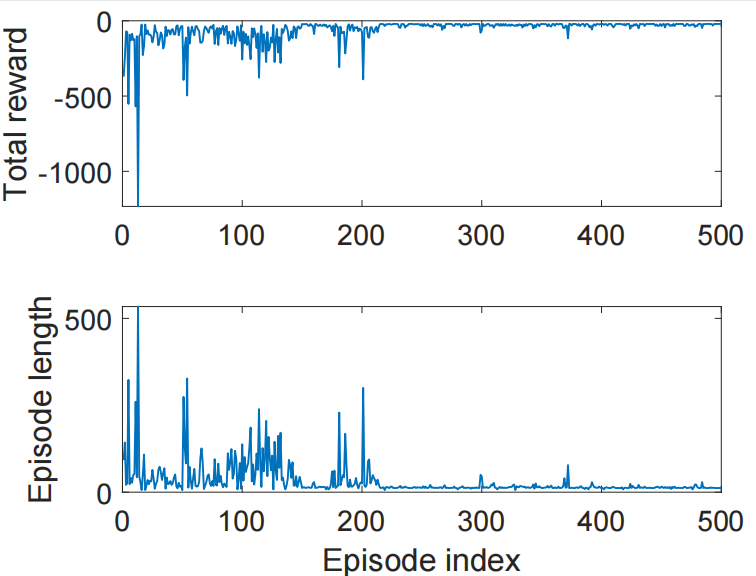
\includegraphics[width=\linewidth]{assets/valuesarsaepisode.jpg}
        \end{minipage}
        \hspace{1cm}
        \begin{minipage}{0.3\textwidth}
            \centering
            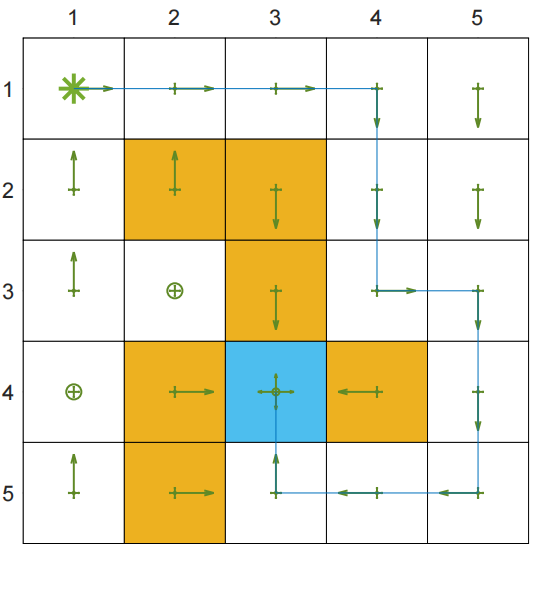
\includegraphics[width=\linewidth]{assets/valuesarsapolicy.jpg}
        \end{minipage}
    \end{center}
    
\end{frame}

\begin{frame}{值近似Q-Learning算法}
    与Sarsa类似,Q-Learning也可以通过值近似推广。

    值近似Q-Learning算法:
    \alert{\[
        w_{t+1}=w_t+\alpha_t\left[r_{t+1}+\gamma \underset{a\in \mathcal{A}(s_{t+1})}{\max}\hat{q}(s_{t+1},a,w_t)-\hat{q}(s_t,a_t,w_t)\right]\nabla_w\hat{q}(s_t,a_t,w_t)
    \]}
    和之前的值近似Sarsa算法几乎一样,只是把$\hat{q}(s_{t+1},a_{t+1},w_t)$替换成了$\underset{a\in \mathcal{A}(s_{t+1})}{\max}\hat{q}(s_{t+1},a,w_t)$。
\end{frame}

\begin{frame}{值近似Q-Learning算法}
    \begin{algorithmic}[1]
        \State \textbf{初始化:}一个对$w$可微的函数$\hat{q}(s,a,w)$。初始化$w=w_0$。一个初始策略$\pi_0$。
        \State \textbf{目标 :}找到一个让智能体从一个特定的起点$s_0$出发,到达终点的最优策略。
        \For{每一次生成轨迹}
            \State $a_0\leftarrow\pi_0(s_0)$
            \While{$s_t$不是目标状态}
                \State 根据$(s_t,a_t)$收集经验样本$(r_{t+1}, s_{t+1})$
                \State 更新动作价值:

                $w_{t+1}=w_t+\alpha_t[r_{t+1}+\gamma \underset{a\in \mathcal{A}(s_{t+1})}{\max}\hat{q}(s_{t+1},a,w_t)-\hat{q}(s_t,a_t,w_t)]\nabla_w\hat{q}(s_t,a_t,w_t)$
                \State 更新策略:
                \[
                    \pi(a|s_t)=\begin{cases}
                        1-\frac{\epsilon}{|\mathcal{A}|}(|\mathcal{A}|-1),\quad a=\arg\max_{a}\hat{q}(s_t,a,w_{t+1}) \\
                        \frac{\epsilon}{|\mathcal{A}|},\quad a \neq \arg\max_{a}\hat{q}(s_t,a,w_{t+1})
                    \end{cases}
                \]
                \State $s_{t+1}\leftarrow s_t$,$a_{t+1}\leftarrow a_t$
            \EndWhile
        \EndFor
    \end{algorithmic}
\end{frame}

\begin{frame}{值近似Q-Learning算法}
    例子:
    \begin{itemize}
        \item 使用\alert{线性函数}进行值近似的Q-Learning:$\hat{q}(s,a,w)=\phi^T(s,a)w$
        \item $\gamma=0.9,\epsilon=0.1,r_\text{boundary}=r_\text{forbidden}=-10, r_\text{target}=1,\alpha=0.001$
    \end{itemize}
    \begin{center}
        \begin{minipage}{0.3\textwidth}
            \centering
            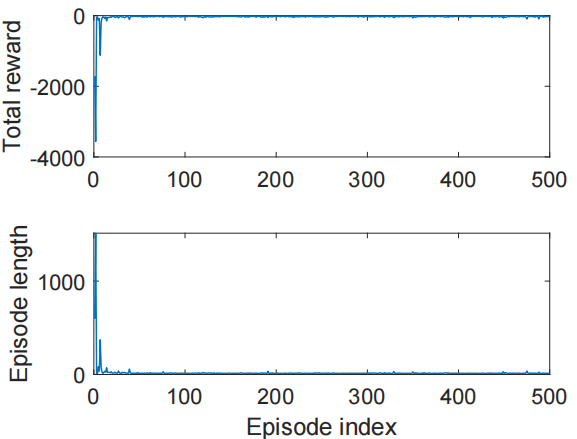
\includegraphics[width=\linewidth]{assets/valueqlearningepisode.png}
        \end{minipage}
        \hspace{1cm}
        \begin{minipage}{0.3\textwidth}
            \centering
            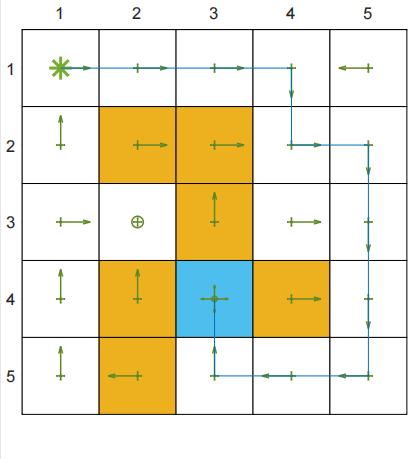
\includegraphics[width=\linewidth]{assets/valueqlearningpolicy.png}
        \end{minipage}
    \end{center}
    
\end{frame}

\begin{frame}{Deep Q-Learning}
    \begin{itemize}
        \item 最早将神经网络与强化学习的结合的算法之一(不是第一)。
        \item 其中神经网络的作用是作为一个非线性方程的拟合器
        \item 与下列算法不同:
        \[
            w_{t+1}=w_t+\alpha_t\left[r_{t+1}+\gamma \underset{a\in \mathcal{A}(s_{t+1})}{\max}\hat{q}(s_{t+1},a,w_t)-\hat{q}(s_t,a_t,w_t)\right]\nabla_w\hat{q}(s_t,a_t,w_t)
        \]
        因为训练神经网络的方式与之前的方法不同。
    \end{itemize}
\end{frame}

\begin{frame}{Deep Q-Learning}
    Deep Q-Learning的目标函数(损失函数):
    \[
        \begin{aligned}
            w_{t+1}&=w_t+\alpha_t\left[\alert{r_{t+1}+\gamma \underset{a\in \mathcal{A}(s_{t+1})}{\max}\hat{q}(s_{t+1},a,w_t)-\hat{q}(s_t,a_t,w_t)}\right]\nabla_w\hat{q}(s_t,a_t,w_t)\\
            &\downdownarrows \\
            J(w)&=\mathbbm{E}\left[\alert{\left(R+\gamma \underset{a\in \mathcal{A}(s_{t+1})}{\max}\hat{q}(S',a,w)-\hat{q}(S,A,w)\right)^2}\right]\\
        \end{aligned}
    \]
    其中$(S,A,R,S')$都是随机变量。
\end{frame}

\begin{frame}{Deep Q-Learning}
    如何最小化这个目标函数?梯度下降法!
    \begin{itemize}
        \item 如何计算目标函数的梯度?
        \item 目标函数:
        \[
            J(w)=\mathbbm{E}\left[\left(R+\gamma \underset{a\in \mathcal{A}(S')}{\max}\hat{q}(S',a,w)-\hat{q}(S,A,w)\right)^2\right]
        \]
        其中参数$w$不但出现在了$\hat{q}(S,A,w)$中,还出现在了
        \[
            y\doteq R+\gamma\underset{a\in \mathcal{A}(S')}{\max}\hat{q}(S',a,w)
        \]
        \item 但是
        \[
            \nabla_wy\alert{\neq} \gamma\underset{a\in \mathcal{A}(S')}{\max}\nabla_w\hat{q}(S',a,w)
        \]
        \item 为了解决这个问题,我们可以假设在$y$中的$w$是不变的(至少对于一段短时间来说,比如5-10个经验样本)。
    \end{itemize}
\end{frame}

\begin{frame}{Deep Q-Learning}
    为了解决这个问题,我们可以引入两个神经网络:
    \begin{itemize}
        \item 一个是\textcolor{blue}{主网络$\hat{q}(s,a,w)$}
        \item 另一个是\alert{目标网络$\hat{q}(s,a,w_T)$}
    \end{itemize}
    如此,我们可以将目标函数可以退化为:
    \[
        J=\mathbbm{E}\left[\left(R+\gamma \underset{a\in \mathcal{A}(S')}{\max}\alert{\hat{q}(S',a,w_T)}-\textcolor{blue}{\hat{q}(S,A,w)}\right)^2\right]
    \]
    其中$w_T$是目标网络中的参数。

    当$w_T$固定时,$J$的梯度就可以按照以下公式计算了:
    \[
        \nabla_wJ=-2\mathbbm{E}\left[\left(R+\gamma \underset{a\in \mathcal{A}(S')}{\max}\alert{\hat{q}(S',a,w_T)}-\textcolor{blue}{\hat{q}(S,A,w)}\right) \textcolor{blue}{\nabla_w\hat{q}(S,A,w)}\right]
    \]
    Deep Q-Learning的基本思想就是使用梯度下降法最小化目标函数。
\end{frame}

\begin{frame}{Deep Q-Learning——双网络}
    \textbf{改进点1:}\alert{双网络,一个目标网络和一个主网络}

    \textbf{实现方式}:
    \begin{itemize}
        \item 令$w$和$w_T$分别是主网络和目标网络的参数,将它们初始化为一样的值。
        \item 每一轮迭代时,从经验池中取出一小批经验样本$\{(s,a,r,s')\}$
        \item 对于其中的每一个经验样本$(s,a,r,s')$计算目标值:
        \[
            y_T\doteq r+\gamma \underset{a\in \mathcal{A}(s_{S'})}{\max}\hat{q}(s',a,w_T)
        \]
        \item 得到一小批数据:$\{(s,a,y_T)\}$
        \item 用$\{(s,a,y_T)\}$训练主网络最小化$(y_T-\hat{q}(s,a,w))^2$
    \end{itemize}
\end{frame}

\begin{frame}{Deep Q-Learning——经验重放}
    \textbf{改进点2:}\alert{经验重放}

    \textbf{什么是经验重放?}

    \textbf{实现方式}:
    \begin{itemize}
        \item 在我们采集了足够多的经验样本之后,我们\alert{并不按照采集他们的顺序去使用它们}。
        \item 而是把它们存在一个叫做\alert{经验池}的集合中\alert{$\mathcal{B}\doteq\{(s,a,r,s')\}$}
        \item 每当我们需要一小批数据的时候,我们就从这个集合中进行随机采样
        \item 我们的采样应该遵循均匀分布。(?)
    \end{itemize}
\end{frame}

\begin{frame}{Deep Q-Learning}
    \begin{algorithmic}[1]
        \State \textbf{初始化:}两个具有相同初始参数的网络$w$和$w_T$。
        \State \textbf{目标 :}从一个任意策略$\pi_b$出发学习出所有的最优动作价值。
        \State 将$\pi_b$产生的经验样本存入经验池$\mathcal{B}=\{(s,a,r,s')\}$
        \For{每一次迭代}
            \State 从$\mathcal{B}$中按照均匀分布采样出一小批经验样本
            \For{每一个经验样本$(s,a,r,s')$}
                \State 使用目标网络计算最优动作价值$y_T= r+\gamma \underset{a\in \mathcal{A}(s_{S'})}{\max}\hat{q}(s',a,w_T)$
            \EndFor
            \State 使用这一小批数据更新主网络,使得$(y_T-\hat{q}(s,a,w))^2$最小
            \State 每过$k$轮将$w_T$设置为$w$。
        \EndFor
    \end{algorithmic}
    \begin{itemize}
        \item 为什么没有策略更新环节?
        \item 与论文中的输入输出有所不同。
    \end{itemize}
\end{frame}

\begin{frame}{Deep Q-Learning}
    例子:
    \begin{itemize}
        \item 只用了\alert{一条}轨迹来生成经验样本。
        \item 这条轨迹有1000步。
        \item 产生这条轨迹的策略就是在每一个状态都均匀的随机选择一个动作。
        \item 使用的神经网络只有一层隐藏全连接层+非线性激活函数用来拟合$\hat{q}(s,a,w)$,这一层有100个神经元。
    \end{itemize}
\end{frame}

\begin{frame}{Deep Q-Learning}
    \begin{center}
        \begin{minipage}{0.18\textwidth}
            \centering
            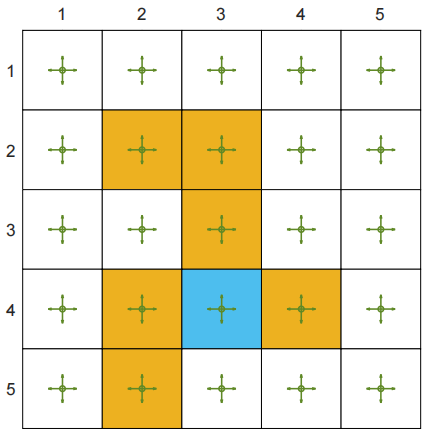
\includegraphics[width=\linewidth]{assets/DQN100behavior.png}
            \captionof{figure}{行为策略}
        \end{minipage}
        \hspace{1cm}
        \begin{minipage}{0.18\textwidth}
            \centering
            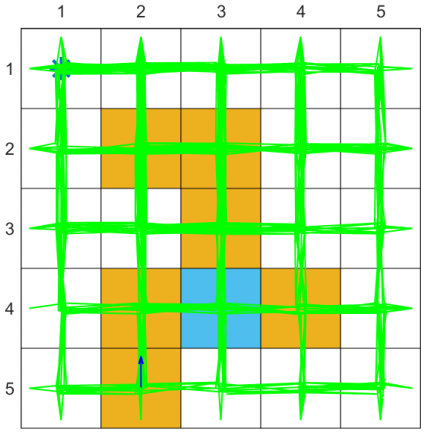
\includegraphics[width=\linewidth]{assets/DQN1000episode.png}
            \captionof{figure}{轨迹}
        \end{minipage}
        \hspace{1cm}
        \begin{minipage}{0.18\textwidth}
            \centering
            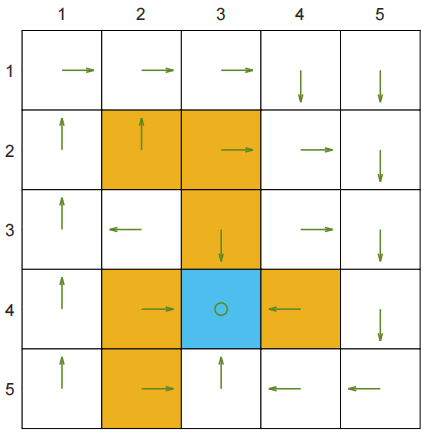
\includegraphics[width=\linewidth]{assets/DQN1000policy.png}
            \captionof{figure}{习得策略}
        \end{minipage}
    \end{center}
    \begin{center}
        \begin{minipage}{0.22\textwidth}
            \centering
            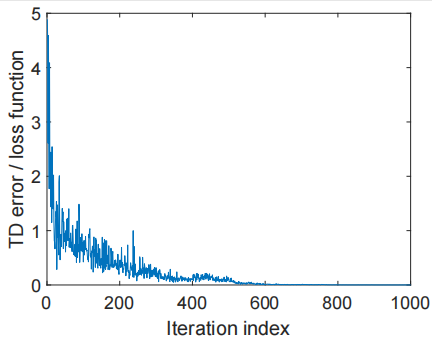
\includegraphics[width=\linewidth]{assets/DQN1000TDerror.png}
            \captionof{figure}{TD Error}
        \end{minipage}
        \hspace{1cm}
        \begin{minipage}{0.22\textwidth}
            \centering
            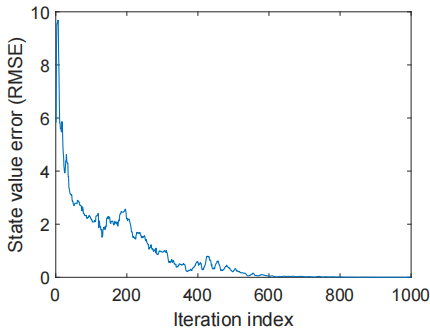
\includegraphics[width=\linewidth]{assets/DQN1000statevalueerror.png}
            \captionof{figure}{状态价值误差}
        \end{minipage}
    \end{center}
\end{frame}


\begin{frame}{Deep Q-Learning}
    如果只有100步呢?
    \begin{center}
        \begin{minipage}{0.18\textwidth}
            \centering
            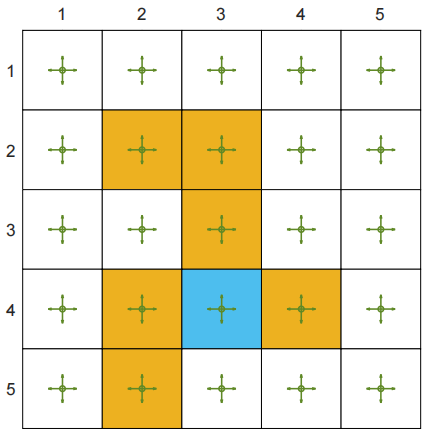
\includegraphics[width=\linewidth]{assets/DQN100behavior.png}
            \captionof{figure}{行为策略}
        \end{minipage}
        \hspace{1cm}
        \begin{minipage}{0.18\textwidth}
            \centering
            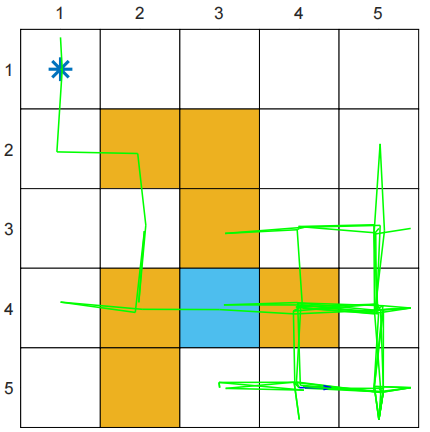
\includegraphics[width=\linewidth]{assets/DQN100episode.png}
            \captionof{figure}{轨迹}
        \end{minipage}
        \hspace{1cm}
        \begin{minipage}{0.18\textwidth}
            \centering
            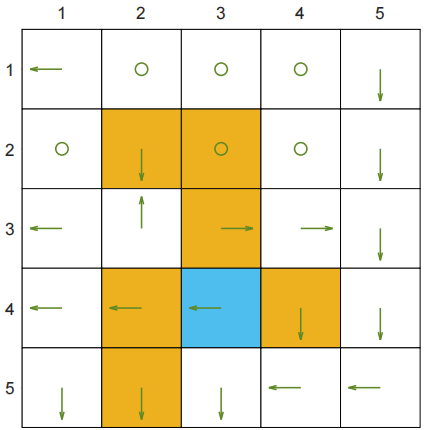
\includegraphics[width=\linewidth]{assets/DQN100policy.png}
            \captionof{figure}{习得策略}
        \end{minipage}
    \end{center}
    \begin{center}
        \begin{minipage}{0.22\textwidth}
            \centering
            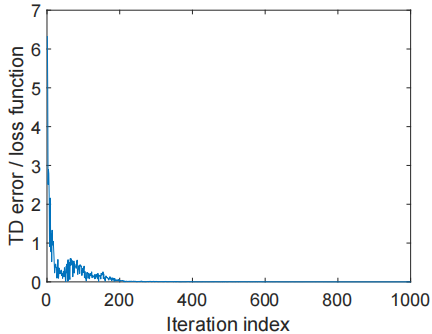
\includegraphics[width=\linewidth]{assets/DQN100TDerror.png}
            \captionof{figure}{TD Error}
        \end{minipage}
        \hspace{1cm}
        \begin{minipage}{0.22\textwidth}
            \centering
            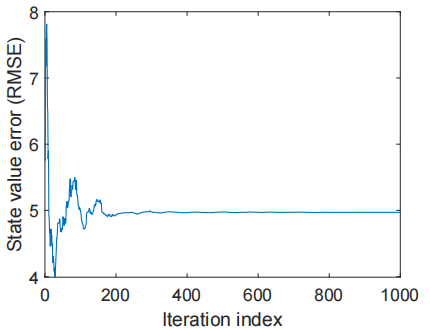
\includegraphics[width=\linewidth]{assets/DQN100statevalueerror.png}
            \captionof{figure}{状态价值误差}
        \end{minipage}
    \end{center}
\end{frame}

\begin{frame}{小结}
    值近似方法:
    \begin{itemize}
        \item 值近似TD算法
        \[
            w_{t+1}=w_t+\alpha_t(r_{t+1}+\gamma \hat{v}(s_{t+1},w_t)-\hat{v}(s_t,w_t))\nabla_w\hat{v}(s_t,w_t)
        \]
        \item 值近似Sarsa算法
        \[
            w_{t+1}=w_t+\alpha_t[r_{t+1}+\gamma \hat{q}(s_{t+1},a_{t+1},w_t)-\hat{q}(s_t,a_t,w_t)]\nabla_w\hat{q}(s_t,a_t,w_t)
        \]
        \item 值近似Q-Learning算法
        \[
            w_{t+1}=w_t+\alpha_t\left[r_{t+1}+\gamma \underset{a\in \mathcal{A}(s_{t+1})}{\max}\hat{q}(s_{t+1},a,w_t)-\hat{q}(s_t,a_t,w_t)\right]\nabla_w\hat{q}(s_t,a_t,w_t)
        \]
        \item Deep Q-Learning
        \begin{itemize}
            \item 双网络
            \item 经验重放
        \end{itemize}
    \end{itemize}
\end{frame}

\end{section}